% Requires \usepackage{booktabs}
% Requires \usepackage{graphicx}

% TODO: Replace the placeholder citation keys below with the actual bibliography keys in your manuscript.

\section{Introduction}
Resource-constrained intrusion detection is increasingly required in wireless, mobile, and telemetry-driven environments where observation quality cannot be guaranteed. UAV-assisted networks and FANET-style deployments are representative examples because they combine dynamic topology, intermittent links, and limited onboard compute, but the underlying problem is broader than UAVs alone: in many operational IDS settings, groups of structured features can be missing, delayed, or corrupted at inference time \cite{uav_security_survey,fanet_security_survey,lightweight_ids_survey}. An IDS that performs well only under clean observations is therefore of limited practical value in deployment-oriented settings.

Much of the recent IDS literature emphasizes clean-set benchmark accuracy through stronger feature engineering, deeper neural models, or transformer-style architectures \cite{deep_ids_survey,transformer_ids_survey}. However, these results do not directly answer the deployment question considered here: whether a lightweight structured detector can preserve discriminative power when informative features are partially missing or corrupted. In this paper, the primary concern is not universal clean-set superiority, but robustness to structured observation loss under realistic resource constraints. This problem is scientifically useful because it is both practically important and empirically under-specified: many papers report stronger architectures, but comparatively few isolate structured missingness as the core deployment failure mode and test it under a controlled, fairness-aligned protocol.

To study this question, we focus on a lightweight structured pipeline rather than heavier pretraining or large-model adaptation. Our method, \textbf{MLP MaskAug}, keeps the same inference-time architecture as a plain multilayer perceptron while changing only the training distribution through random masking, block masking, and mild proportional noise. This design targets a concrete failure mode---partial observation loss---without increasing inference-time complexity. We additionally retain a fair aligned lexical baseline, TF-IDF + Logistic Regression, because compact textified flow records can be highly competitive on curated benchmarks once they are discretized into lexical tokens. The contribution is therefore not a new large architecture, but a deployment-oriented training strategy for making a small structured detector substantially more reliable under missing observations. Precisely because the backbone is simple, any robustness gain is easier to attribute to the proposed training strategy itself rather than to hidden capacity increases, which makes the resulting evidence more interpretable for practical IDS design.

The empirical study is intentionally structured around two complementary questions. First, on a curated seven-class UNSW-NB15 benchmark, we test whether missingness-aware augmentation reliably strengthens the lightweight structured baseline after text and structured models are aligned to the same capped split. Second, on binary CICIDS2017, we test whether the same trend transfers beyond the primary benchmark. The resulting picture is more nuanced than a typical ``best-model'' story: on fairness-aligned UNSW-NB15, sparse lexical baselines remain stronger in absolute Macro-F1, but \textbf{MLP MaskAug} consistently improves over the plain MLP under every reported degradation family; on CICIDS2017, the same structured method becomes the strongest model under every reported condition. This benchmark dependence is not a weakness to hide. It is part of the paper's main message: representation choice and robustness behavior must be evaluated under fair comparison rather than assumed from model family alone.

The contribution of this work is therefore narrower but more defensible than universal superiority. Specifically:
\begin{itemize}
\item We formulate structured observation loss as a first-class deployment problem for lightweight intrusion detection, rather than treating robustness as a generic afterthought to clean-set accuracy.
\item We propose \textbf{MLP MaskAug}, a missingness-aware augmentation strategy for a lightweight structured IDS pipeline that preserves the inference-time model architecture of a plain MLP while substantially improving its degradation tolerance.
\item We conduct a fairness-aligned robustness study on UNSW-NB15 and show that the proposed method yields stable gains over the plain MLP, with the largest improvements appearing under structured feature missingness and exact one-sided Wilcoxon support across nine paired runs.
\item We provide external validation on CICIDS2017 and show that the relative ranking between lexical and structured methods is benchmark-dependent, while the robustness benefit of the proposed structured training strategy remains practically meaningful.
\end{itemize}

\section{Related Work}
\subsection{Lightweight IDS for Resource-Constrained Environments}
Lightweight intrusion detection has been studied in resource-constrained environments such as IoT systems, wireless edge networks, and UAV/FANET deployments, where inference cost, memory footprint, and operational simplicity are often as important as raw benchmark accuracy \cite{lightweight_ids_survey,edge_ids_survey,uav_fanet_ids_survey}. Existing work spans compact multilayer perceptrons, lightweight CNN or recurrent hybrids, distributed detectors, and federated or cooperative designs. These studies establish the deployment motivation for this paper, but they often emphasize architectural efficiency more than robustness under partial observation loss. In other words, lightweight IDS work still under-specifies what happens when the detector receives incomplete structured inputs at inference time.

\subsection{Robust Intrusion Detection under Missing or Corrupted Features}
A related literature seeks to improve IDS reliability under noisy or shifting conditions through feature selection, imputation, augmentation, ensemble methods, or more expressive temporal architectures \cite{robust_ids_missing_data,missing_data_ids_survey,distribution_shift_ml}. This line of work is important, but it often mixes several failure modes together, including noise, distribution shift, imbalance, and adversarial perturbation. The present paper isolates a more specific deployment problem: structured feature missingness, including both independent feature loss and grouped block loss. Our emphasis is therefore not on general robustness as a broad slogan, but on whether degradation-aware training can materially strengthen a lightweight structured detector under partial observation failure.

\subsection{Structured versus Text-Based Flow Representations}
Recent cybersecurity work has also explored textified or sequence-style representations of security telemetry, including BERT-style encoders, log-language models, and other structured-to-text pipelines \cite{textified_security_telemetry,bert_for_ids,llm_for_security_telemetry}. These studies show that serialized records can preserve useful discriminative information, but they often emphasize pretrained encoders, synthetic-data pipelines, or language-model adaptation. By contrast, the current results show that even sparse lexical baselines can be unexpectedly strong once curated flow features are discretized into compact tokens. This observation is not a reason to dismiss text-based representations; rather, it sharpens the comparison target. The key question is not whether text works, but when a missingness-aware structured pipeline is more reliable than a lexical alternative under controlled corruption. Existing representation work rarely addresses that question through fair split alignment and corruption-aware evaluation against lightweight structured models.

\section{Method}
\subsection{Problem Setting}
We study lightweight intrusion detection from structured network-flow records under partial observation loss and feature corruption. Each sample is represented as a mixed-type feature vector $\mathbf{x}\in\mathbb{R}^{d}$ with label $y \in \{0,\dots,C-1\}$, where $C=7$ for the main UNSW-NB15 study and $C=2$ for the CICIDS2017 external validation. The goal is not only to maximize clean-set performance, but also to preserve discriminative power when informative numerical features are missing or perturbed.

\subsection{Structured and Text Baselines}
The plain structured baseline is a two-hidden-layer MLP with hidden sizes $(512,256)$, ReLU activations, and dropout $p=0.2$. Categorical features are imputed with a constant \texttt{UNK} token and one-hot encoded. Numerical features are imputed with zeros, augmented with missing-value indicators, and standardized. The model is trained with class-weighted cross-entropy, where the weight for class $c$ is
\[
w_c = \frac{N}{C \cdot n_c},
\]
with $N$ the number of training samples, $C$ the number of classes, and $n_c$ the number of training samples in class $c$. Optimization uses Adam with learning rate $10^{-3}$, weight decay $10^{-4}$, batch size $512$, gradient clipping at $5.0$, a maximum of $20$ epochs, and early stopping patience $5$.

The text baselines serialize each flow as a compact \texttt{key=value} sequence and apply TF-IDF features followed by a linear classifier. We report both TF-IDF + Logistic Regression and TF-IDF + SVM on the clean benchmark. In the robustness figures, TF-IDF + Logistic Regression is used as the main lexical comparator because it is the strongest aligned sparse baseline on the primary UNSW benchmark. The TF-IDF configuration is fixed to unigram--bigram features, \texttt{max\_features}$=50000$, \texttt{min\_df}$=1$, \texttt{max\_df}$=1.0$, \texttt{norm}$=\ell_2$, \texttt{use\_idf=True}, \texttt{smooth\_idf=True}, and \texttt{sublinear\_tf=False}. Logistic regression uses \texttt{solver=saga}, \texttt{max\_iter=2000}, and \texttt{class\_weight=balanced}. Linear SVM uses \texttt{C=1.0} and \texttt{class\_weight=balanced}.

\subsection{Proposed Method: MLP MaskAug}
Our final method, denoted \texttt{MLP MaskAug}, keeps the same inference-time MLP architecture but augments the structured training distribution with three degradation-aware transformations selected by a sensitivity study: random masking with ratios $0.1$ and $0.3$, block masking with ratio $0.1$, and mild multiplicative noise with ratio $0.1$. Let $\mathcal{D}$ denote the clean training set and $\mathcal{N}$ the set of numerical features. The augmented training set is
\[
\mathcal{D}_{\mathrm{aug}} =
\mathcal{D}
\cup \mathcal{T}_{\mathrm{mask}}(\mathcal{D})
\cup \mathcal{T}_{\mathrm{block}}(\mathcal{D})
\cup \mathcal{T}_{\mathrm{noise}}(\mathcal{D}).
\]
For random masking, each numerical feature is independently set to missing with probability $r$:
\[
x_j' =
\begin{cases}
\mathrm{NaN}, & \text{with probability } r,\\
x_j, & \text{otherwise}.
\end{cases}
\]
For block masking, a correlated feature group $G_k \subseteq \mathcal{N}$ is jointly removed:
\[
\mathbf{x}'_{G_k} = \mathrm{NaN}.
\]
For proportional noise, positive numerical features are perturbed by
\[
x_j' = x_j \cdot (1 + \epsilon), \qquad \epsilon \sim \mathcal{U}(-r, r).
\]
The model is still trained with standard class-weighted cross-entropy. Thus, the contribution comes from missingness-aware training rather than a larger model or a more expensive inference path.

\section{Experiments}
\subsection{Experimental Setup and Fairness Alignment}
The final paper uses two datasets. UNSW-NB15 is the primary benchmark and is evaluated as a seven-class intrusion classification task on the curated 15-feature subset used in the project, consisting of $3$ categorical and $12$ numerical features. The medium-tier structured split contains $21{,}000$ training samples and $15{,}803$ evaluation samples. The training split is balanced at $3000$ samples per class, whereas the evaluation split remains capped but imbalanced; the full per-class counts are reported in Table~\ref{tab:unsw_class_counts} in the appendix. After preprocessing, the structured UNSW input dimension is $162$.

CICIDS2017 is used for external validation in a binary benign-vs-attack setting. Its medium-tier structured split contains $6000$ training samples and $6000$ evaluation samples, with $3000$ benign and $3000$ attack samples in each split. After preprocessing, the final structured input dimension is $80$. Table~\ref{tab:protocol} summarizes the dataset transparency information used throughout the paper.

\begin{table}[t]
\centering
\caption{Dataset and protocol transparency summary for the final experiments.}
\label{tab:protocol}
\resizebox{\linewidth}{!}{%
\begin{tabular}{llccccccl}
\toprule
Dataset & Task & Train & Eval & Train class counts & Eval class counts & $\#$Cat & $\#$Num & Input dim \\
\midrule
UNSW-NB15 & 7-class intrusion classification & 21,000 & 15,803 & 3000 per class & Backdoor 1466 / DoS 3000 / Exploits 3000 / Normal 3000 / Reconnaissance 3000 / Shellcode 1302 / Worms 1035 & 3 & 12 & 162 \\
CICIDS2017 & Binary benign-vs-attack classification & 6,000 & 6,000 & benign 3000 / attack 3000 & benign 3000 / attack 3000 & 0 & 78 & 80 \\
\bottomrule
\end{tabular}%
}
\end{table}

The core comparison retains three primary methods: \texttt{MLP MaskAug}, the plain \texttt{MLP}, and the strongest aligned lexical baseline, TF-IDF + Logistic Regression. TF-IDF + SVM, structured logistic regression, and structured linear SVM are kept as secondary references in the clean comparison table. For fairness, the final UNSW text baseline is rebuilt from the same capped structured split using the same \texttt{source\_row\_id} set and the same train-only discretization rules. This correction is necessary because earlier text baselines had been generated from a different sample pool and therefore were not directly comparable to the structured models.

We evaluate three degradation families. \texttt{E1\_clean} leaves evaluation samples unchanged. \texttt{E3\_mask\_r} randomly masks numerical features at rate $r\%$. \texttt{E3\_block\_r} removes correlated feature groups at rate $r\%$. \texttt{E4\_noise\_r} multiplies positive numerical features by a factor sampled uniformly from $[1-r,1+r]$. On UNSW-NB15, we evaluate the full grid $\{\texttt{Clean}, \texttt{Mask10}, \texttt{Mask30}, \texttt{Mask50}, \texttt{Block10}, \texttt{Block30}, \texttt{Block50}, \texttt{Noise10}, \texttt{Noise30}, \texttt{Noise50}\}$, while the main paper tables and figures focus on the representative 30\% and 50\% settings. On CICIDS2017, the external validation uses the compact grid $\{\texttt{Clean}, \texttt{Mask30}, \texttt{Mask50}, \texttt{Block30}, \texttt{Block50}, \texttt{Noise30}, \texttt{Noise50}\}$.

A representative textified flow record from the aligned UNSW training split is shown below to clarify the lexical input format used by the TF-IDF baselines:
\begin{quote}
\small
\texttt{proto=unas ; state=INT ; service=- ; dur\_cat=low ; spkts\_cat=low ; dpkts\_cat=zero ; sbytes\_cat=low ; dbytes\_cat=zero ; sload\_cat=very\_high ; dload\_cat=zero ; tcprtt\_cat=zero ; synack\_cat=zero ; ackdat\_cat=zero ; ct\_srv\_src\_cat=medium ; ct\_state\_ttl\_cat=low}
\normalsize
\end{quote}

\subsection{Reproducibility, Metrics, and Statistical Testing}
Unless otherwise noted, Macro-F1 is the primary comparison metric and accuracy is retained as a secondary descriptive metric. This choice is necessary because the main UNSW-NB15 evaluation split remains class-imbalanced even after medium-tier capping. The main UNSW clean and robustness tables are reported on the fixed split with split seed $42$. A separate split-stability analysis uses split seeds $\{42,52,62\}$ and model seeds $\{11,21,31\}$, yielding $n=9$ paired structured runs. The TF-IDF baselines are deterministic under a fixed text bundle and therefore do not rely on random initialization; their split-level reruns are used only to verify consistency under matched partitions.

Statistical testing is reserved for the paired comparison between \texttt{MLP MaskAug} and the plain \texttt{MLP}, since the main scientific question is whether degradation-aware structured training yields consistent gains over its non-augmented counterpart. We use the exact one-sided Wilcoxon signed-rank test on the nine paired observations for each reported condition. In the final results, all paired gains are positive, so the reported $p$-values share the same minimum attainable exact value.

Lightweight evidence is measured directly rather than inferred only from parameter counts. All efficiency measurements are taken on a workstation with a 12th Gen Intel Core i9-12900KS CPU, an NVIDIA GeForce RTX 3090 Ti GPU, and approximately $32$ GB of RAM. The reported latency and throughput values are CPU inference measurements. The final lightweight measurement environment used CPU-only PyTorch, so GPU memory is reported as \texttt{N/A} in Table~\ref{tab:efficiency}.

\section{Results and Discussion}
\subsection{Fair Main Results on UNSW-NB15}
After aligning the text and structured baselines to the same capped UNSW split and the same curated feature subset, the sparse lexical baselines become substantially stronger than previously estimated. Table~\ref{tab:main_clean} shows that the strongest clean result now comes from TF-IDF + Logistic Regression at $0.7723$, followed by TF-IDF + SVM at $0.7636$. The proposed \texttt{MLP MaskAug} reaches $0.7036$, improving over the plain MLP at $0.6766$ but not surpassing the aligned lexical baselines. This correction should not be hidden, because it changes the interpretation of the benchmark: the compact discretized text representation turns the curated UNSW task into a highly lexical classification problem.

\begin{table}[t]
\centering
\caption{Fair clean-set comparison on UNSW-NB15 after aligning the text and structured baselines to the same capped split and curated feature subset.}
\label{tab:main_clean}
\begin{tabular}{lccc}
\toprule
Method & Input type & Macro-F1 & Trainable params \\
\midrule
TF-IDF + Logistic Regression & Text & 0.7723 & 4,137 \\
TF-IDF + SVM & Text & 0.7636 & 4,137 \\
MLP MaskAug & Structured & 0.7036 & 216,583 \\
MLP & Structured & 0.6766 & 216,583 \\
Structured Logistic Regression & Structured & 0.5121 & 1,141 \\
Structured Linear SVM & Structured & 0.4766 & 1,141 \\
\bottomrule
\end{tabular}
\end{table}

The aligned robustness results are summarized in Table~\ref{tab:unsw_robustness} and Figures~\ref{fig:unsw_curve}--\ref{fig:gain_over_mlp}. On UNSW-NB15, the aligned TF-IDF + Logistic Regression baseline remains strongest in absolute Macro-F1 across all seven reported conditions. At \texttt{Mask30}, for instance, it reaches $0.6752$, compared with $0.6019$ for \texttt{MLP MaskAug} and $0.4675$ for the plain \texttt{MLP}. At \texttt{Block30}, the corresponding values are $0.6566$, $0.6142$, and $0.5157$. The lexical baseline also remains strongest under the two reported noise settings.

This does \emph{not} make the proposed method unimportant. Rather, it sharpens the contribution of the paper. \texttt{MLP MaskAug} does not universally dominate every baseline, but it consistently and materially improves the structured pipeline over the plain MLP under every reported degradation family. The gain over the plain MLP is $0.1414$ at \texttt{Mask30}, $0.1799$ at \texttt{Mask50}, $0.1074$ at \texttt{Block30}, and $0.1460$ at \texttt{Block50}. Even under noise, the gains remain positive at $0.0376$ and $0.0438$ for \texttt{Noise30} and \texttt{Noise50}, respectively. Figure~\ref{fig:unsw_curve} makes the degradation pattern easier to read by separating random masking, block masking, and noise into aligned panels, while Figure~\ref{fig:gain_over_mlp} converts the same result into an effect-style comparison against the plain MLP.

\begin{table}[t]
\centering
\caption{Fair robustness comparison on UNSW-NB15. The lexical baseline is the aligned TF-IDF + Logistic Regression model built from the same curated structured split.}
\label{tab:unsw_robustness}
\resizebox{\linewidth}{!}{%
\begin{tabular}{lccccccc}
\toprule
Method & Clean & Mask30 & Mask50 & Block30 & Block50 & Noise30 & Noise50 \\
\midrule
MLP MaskAug & 0.7036 & 0.6019 & 0.5522 & 0.6142 & 0.5618 & 0.6288 & 0.5934 \\
MLP & 0.6766 & 0.4675 & 0.3797 & 0.5157 & 0.4219 & 0.5940 & 0.5515 \\
TF-IDF + Logistic Regression & 0.7723 & 0.6752 & 0.5975 & 0.6566 & 0.5812 & 0.6767 & 0.6512 \\
\bottomrule
\end{tabular}%
}
\end{table}

\begin{figure}[t]
    \centering
    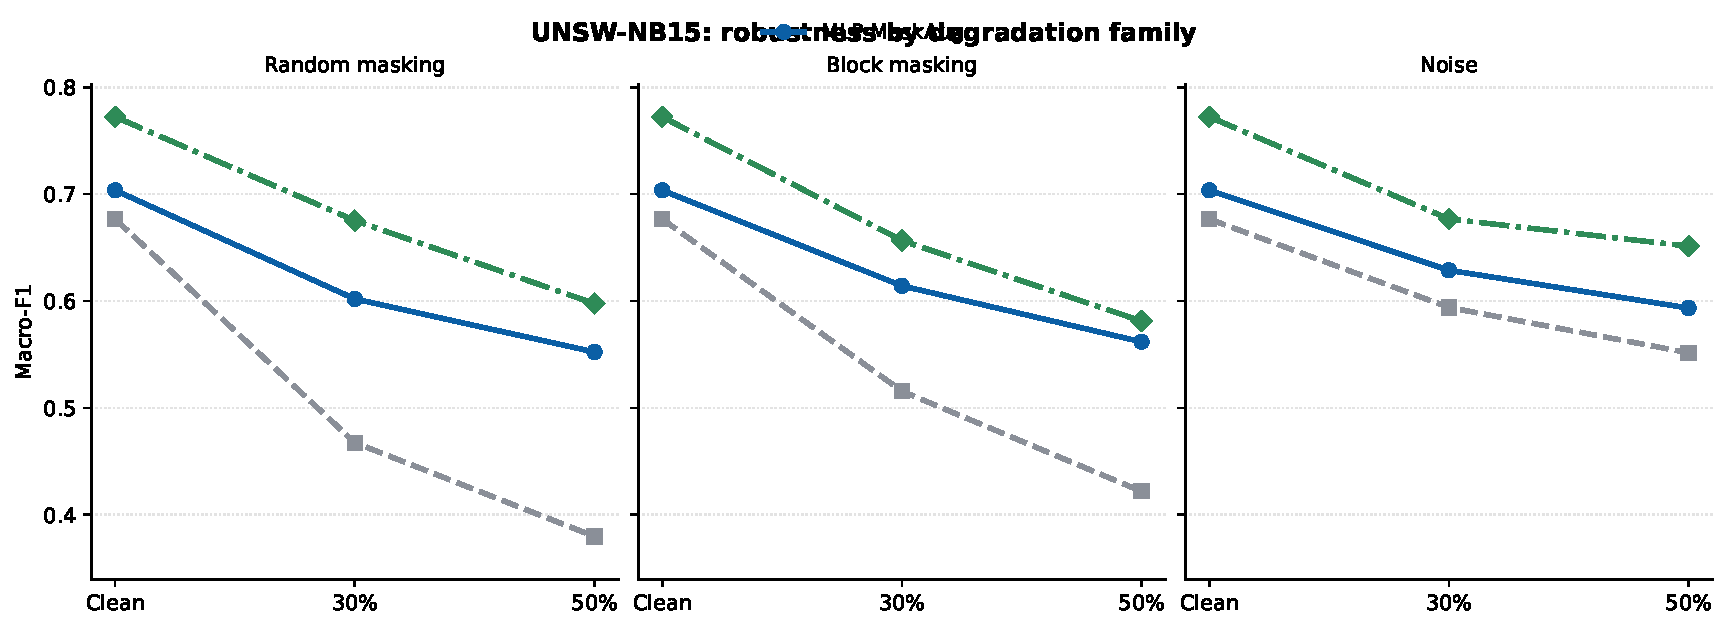
\includegraphics[width=\linewidth]{figures_main/unsw_robustness_curve.pdf}
    \caption{Journal-style multi-panel robustness view on UNSW-NB15. Each panel isolates one degradation family so that the relative behavior under random masking, block masking, and noise can be compared without compressing all conditions into a single long axis.}
    \label{fig:unsw_curve}
\end{figure}

\begin{figure}[t]
    \centering
    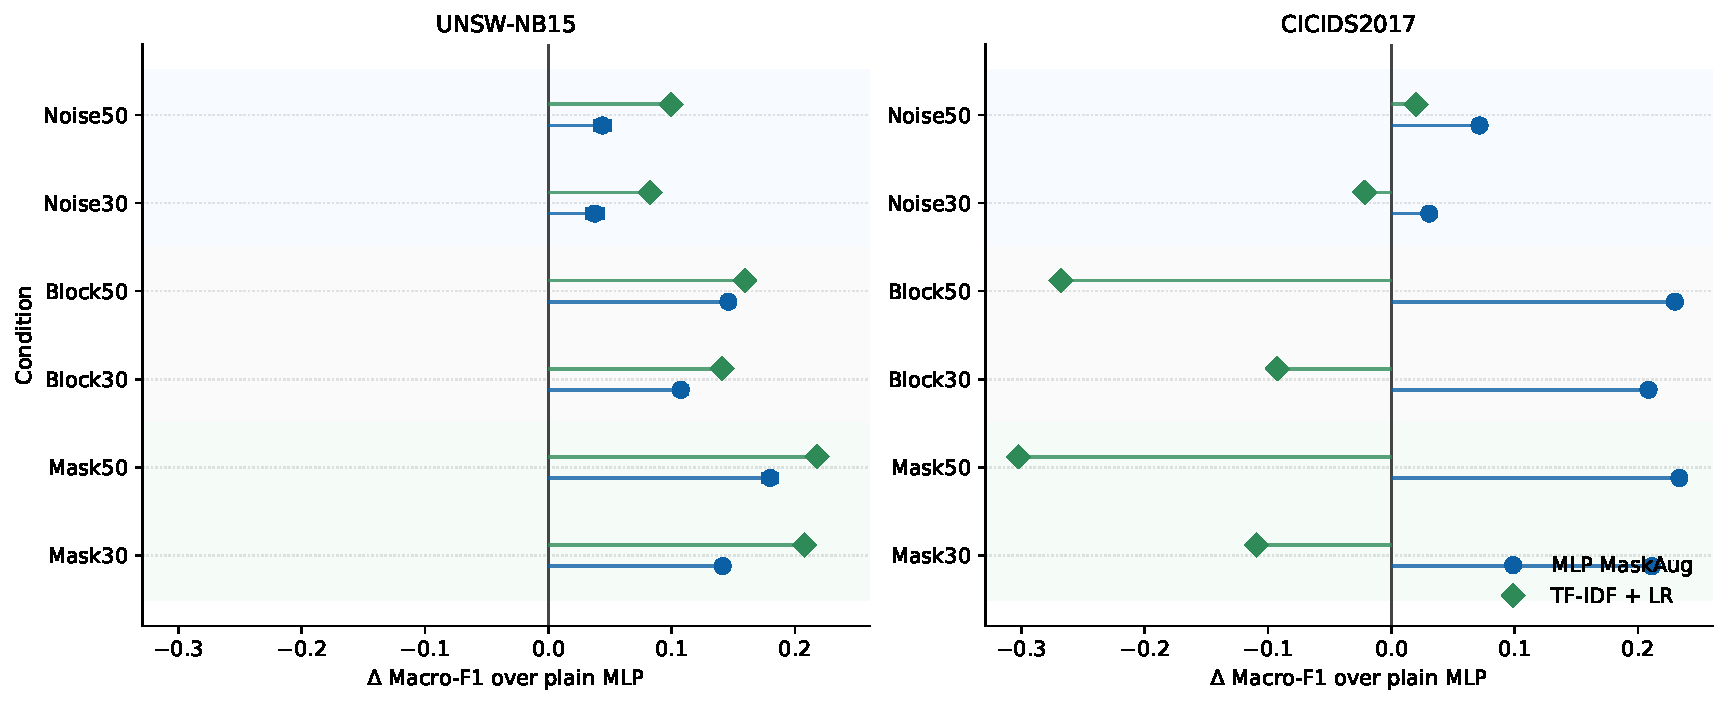
\includegraphics[width=\linewidth]{figures_main/gain_over_mlp.pdf}
    \caption{Effect-style view of Macro-F1 gain over the plain MLP. For UNSW-NB15, \texttt{MLP MaskAug} is shown with the exact $95\%$ confidence intervals derived from the split-stability study.}
    \label{fig:gain_over_mlp}
\end{figure}

Table~\ref{tab:ablation} separates the contribution of the augmentation components. Random masking and block masking are both useful, but they specialize to different corruption families: the MaskOnly variant is strongest under random masking, whereas the BlockOnly variant is strongest under block masking. The combined Mask+Block configuration is more balanced, and the final sensitivity study shows that adding mild training-time noise yields the best four-condition operating point without materially sacrificing clean performance. This selected configuration is reported throughout the paper as \texttt{MLP MaskAug}.

\begin{table}[t]
\centering
\caption{Ablation and selected main configuration on UNSW-NB15. The final paper method is the sensitivity-selected Mask+Block+Noise configuration, reported here as MLP MaskAug.}
\label{tab:ablation}
\resizebox{\linewidth}{!}{%
\begin{tabular}{lccccccc}
\toprule
Variant & Clean & Mask30 & Mask50 & Block30 & Block50 & Noise30 & Noise50 \\
\midrule
MLP & 0.6766 & 0.4675 & 0.3797 & 0.5157 & 0.4219 & 0.5940 & 0.5515 \\
MaskOnly \{0.1,0.3\} & 0.6923 & 0.6118 & 0.5647 & 0.6064 & 0.5562 & 0.6273 & 0.5955 \\
BlockOnly \{0.1\} & 0.6970 & 0.5170 & 0.4606 & 0.6316 & 0.5781 & 0.5986 & 0.5636 \\
Mask+Block & 0.7003 & 0.6102 & 0.5596 & 0.6250 & 0.5736 & 0.6100 & 0.5737 \\
MLP MaskAug & 0.7017 & 0.6135 & 0.5640 & 0.6133 & 0.5577 & 0.6348 & 0.5990 \\
\bottomrule
\end{tabular}%
}
\end{table}

\subsection{Statistical Support, Lightweight Evidence, and External Validation}
Table~\ref{tab:split_significance} shows that the improvement over the plain MLP is stable across three split seeds and three model seeds. The exact one-sided Wilcoxon test yields the same minimum attainable $p$-value, $p = 0.001953125 = 1/512$, under every reported condition because the number of paired observations is $n=9$ and all paired differences are positive. The rank-biserial effect size is therefore $1.0$ throughout. These values do not establish a universal law, but they strongly reduce the risk that the observed gain is a seed artifact.

Table~\ref{tab:efficiency} complements the accuracy results with direct lightweight evidence. The proposed method uses the same inference-time MLP architecture as the plain baseline: it has the same model size on disk (about $0.83$ MB), the same number of trainable parameters ($216{,}583$), and sub-$0.013$ ms CPU latency per sample. The extra cost of the method is concentrated in training rather than deployment, which is consistent with the actual mechanism of the method. Figure~\ref{fig:efficiency_tradeoff} summarizes the same point in trade-off form. On UNSW-NB15, the lexical baseline remains strongest in absolute missingness performance, but it is slower at inference. On CICIDS2017, \texttt{MLP MaskAug} combines the strongest missingness robustness with a compact deployment footprint.

\begin{table}[t]
\centering
\caption{Split-level stability and exact one-sided Wilcoxon statistics on UNSW-NB15. Each row pools nine paired runs (three split seeds $\times$ three model seeds).}
\label{tab:split_significance}
\begin{tabular}{lcccccc}
\toprule
Condition & MLP & MLP MaskAug & Gain & 95\% CI & Effect size & $p$-value \\
\midrule
Clean & 0.6755 & 0.7027 & 0.0272 & [0.0220, 0.0333] & 1.0000 & 0.0019531 \\
Mask30 & 0.4687 & 0.6102 & 0.1414 & [0.1368, 0.1460] & 1.0000 & 0.0019531 \\
Mask50 & 0.3808 & 0.5607 & 0.1799 & [0.1738, 0.1862] & 1.0000 & 0.0019531 \\
Block30 & 0.5121 & 0.6195 & 0.1074 & [0.1022, 0.1125] & 1.0000 & 0.0019531 \\
Block50 & 0.4169 & 0.5629 & 0.1460 & [0.1421, 0.1499] & 1.0000 & 0.0019531 \\
Noise30 & 0.5948 & 0.6324 & 0.0376 & [0.0309, 0.0449] & 1.0000 & 0.0019531 \\
Noise50 & 0.5521 & 0.5960 & 0.0438 & [0.0379, 0.0501] & 1.0000 & 0.0019531 \\
\bottomrule
\end{tabular}
\end{table}

\begin{table}[t]
\centering
\caption{Efficiency comparison on the fair UNSW split (split seed 42, CPU inference mode). The reported MLP MaskAug uses the same inference architecture as the plain MLP.}
\label{tab:efficiency}
\resizebox{\linewidth}{!}{%
\begin{tabular}{lcccccc}
\toprule
Method & Disk size (MB) & Train time (s) & CPU latency (ms) & CPU throughput & Peak CPU RAM (MB) & Peak GPU mem (MB) \\
\midrule
TF-IDF + Logistic Regression & 0.055 & 4.29 & 0.0210 & 47523.5 & 321.9 & N/A \\
TF-IDF + SVM & 0.055 & 0.89 & 0.0211 & 47443.0 & 323.2 & N/A \\
MLP & 0.828 & 6.39 & 0.0048 & 206212.9 & 405.5 & N/A \\
MLP MaskAug & 0.828 & 27.53 & 0.0120 & 82987.6 & 495.2 & N/A \\
\bottomrule
\end{tabular}%
}
\end{table}

\begin{figure}[t]
    \centering
    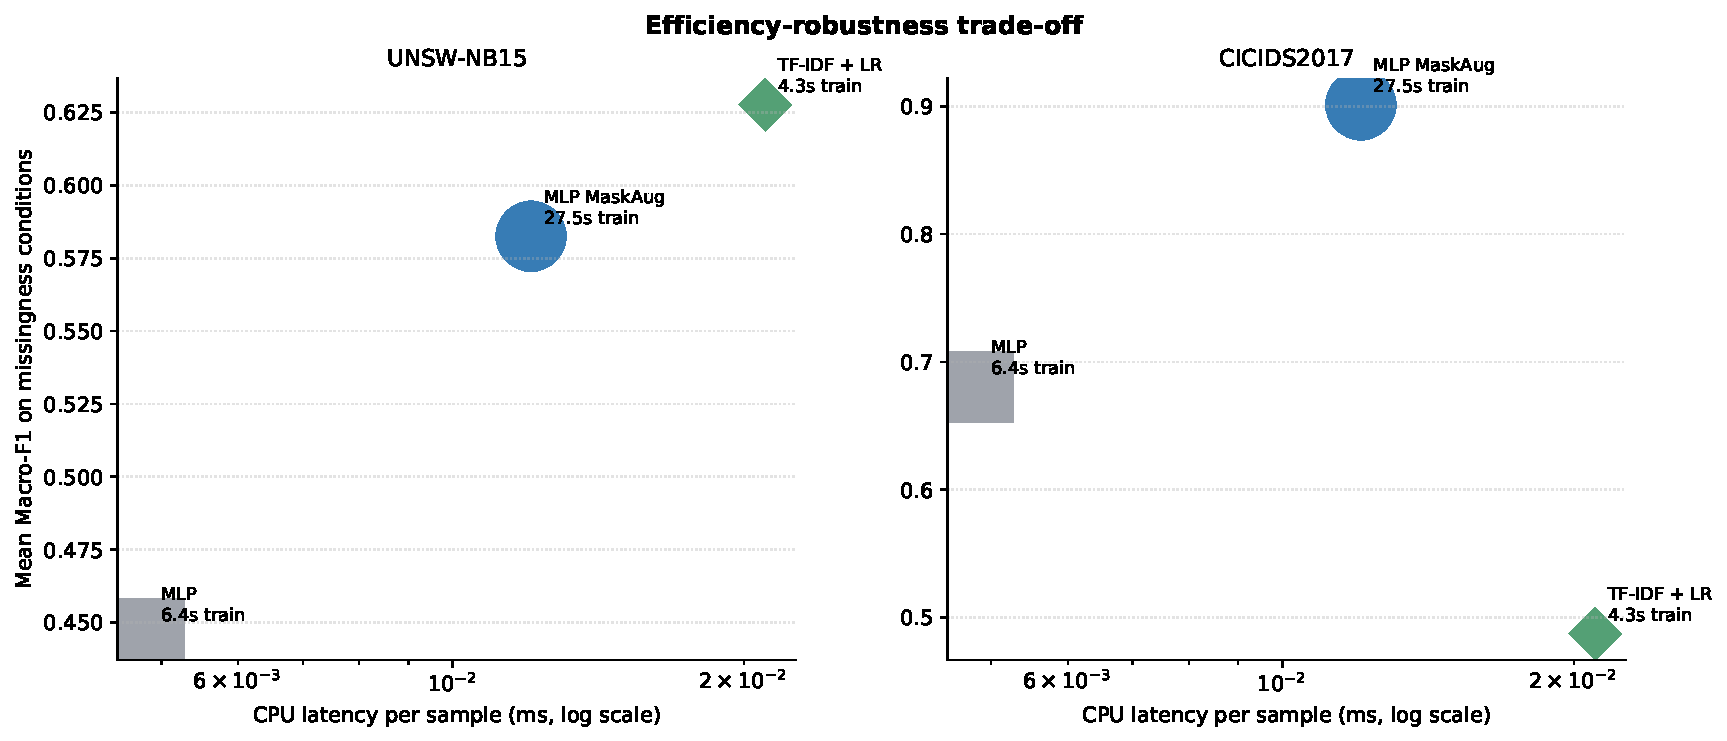
\includegraphics[width=\linewidth]{figures_main/efficiency_tradeoff.pdf}
    \caption{Latency--robustness trade-off. The vertical axis reports the mean Macro-F1 over the missingness conditions \texttt{Mask30}, \texttt{Mask50}, \texttt{Block30}, and \texttt{Block50}; point size reflects model size on disk. Leftward and upward are better.}
    \label{fig:efficiency_tradeoff}
\end{figure}

The external validation results are reported in Table~\ref{tab:cic_external} and Figure~\ref{fig:cic_curve}. Unlike the curated UNSW benchmark, CICIDS2017 does not favor the lexical baseline. The selected \texttt{MLP MaskAug} is strongest under every reported CIC condition, including the clean setting. At \texttt{Mask30}, for instance, it reaches $0.9324$, compared with $0.7212$ for the plain MLP and $0.6116$ for the fair lexical baseline. This cross-dataset shift is scientifically useful because it shows that the relative strength of structured and lexical pipelines is benchmark-dependent rather than universal. The curated UNSW benchmark is unusually favorable to sparse lexical classification once the features are discretized and textified, whereas CICIDS2017 is much more favorable to the structured missingness-aware pipeline.

\begin{table}[t]
\centering
\caption{External validation on CICIDS2017. The lexical baseline is a fair text model built from the same structured CIC split.}
\label{tab:cic_external}
\resizebox{\linewidth}{!}{%
\begin{tabular}{lccccccc}
\toprule
Method & Clean & Mask30 & Mask50 & Block30 & Block50 & Noise30 & Noise50 \\
\midrule
MLP MaskAug & 0.9815 & 0.9324 & 0.8729 & 0.9321 & 0.8673 & 0.9771 & 0.9678 \\
MLP & 0.9697 & 0.7212 & 0.6393 & 0.7235 & 0.6374 & 0.9463 & 0.8964 \\
TF-IDF + Logistic Regression & 0.9478 & 0.6116 & 0.3370 & 0.6311 & 0.3696 & 0.9247 & 0.9163 \\
\bottomrule
\end{tabular}%
}
\end{table}

\begin{figure}[t]
    \centering
    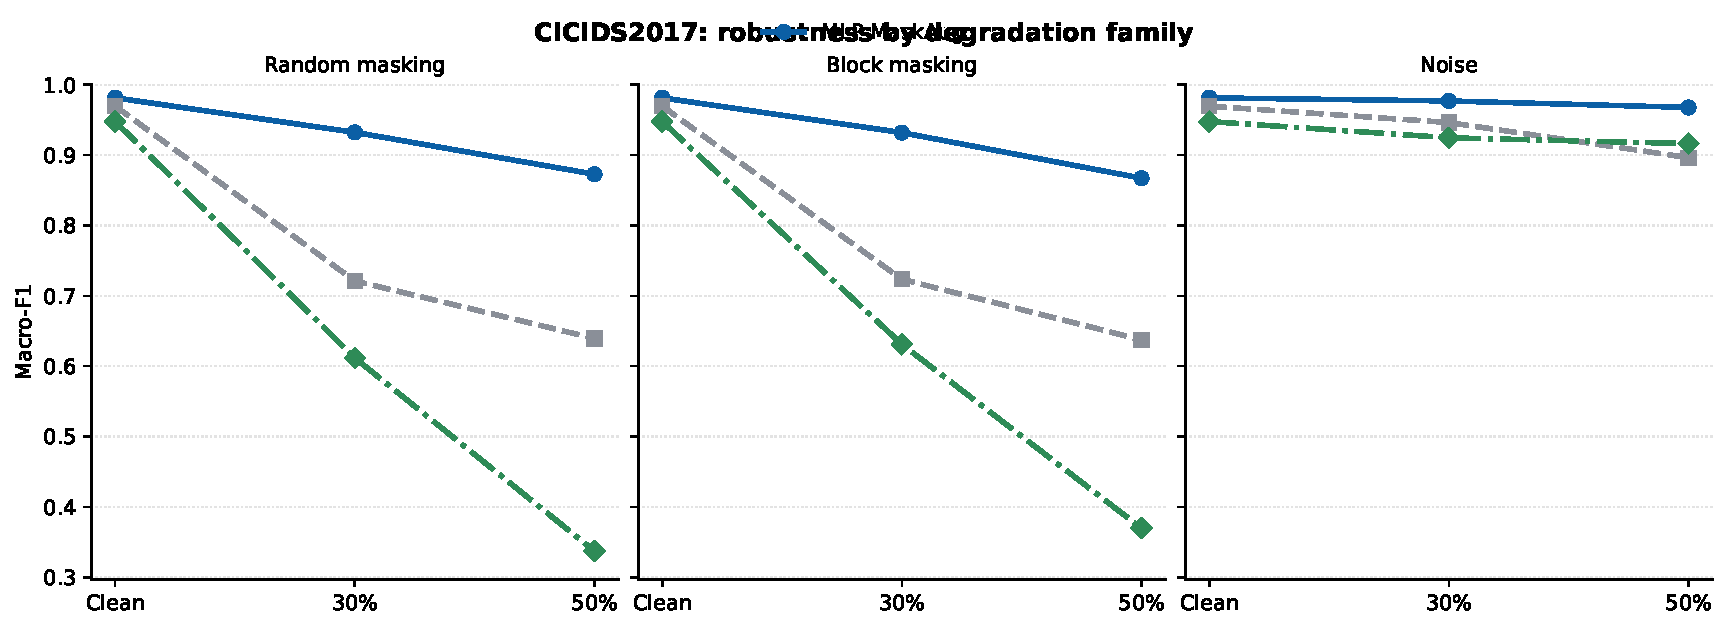
\includegraphics[width=\linewidth]{figures_main/cic_robustness_curve.pdf}
    \caption{Journal-style multi-panel robustness view on CICIDS2017. Unlike UNSW-NB15, the selected structured method is strongest across all three degradation families.}
    \label{fig:cic_curve}
\end{figure}

\subsection{Discussion and Limitations}
The combined evidence supports four restrained conclusions. First, after fairness alignment, the curated UNSW benchmark is dominated by sparse lexical baselines; the proposed structured method does not beat the aligned text models there. Second, the proposed method still yields a statistically stable and practically meaningful gain over the plain MLP, and that gain is largest under missingness. Third, the efficiency analysis shows that the method remains lightweight in the sense that it preserves the same inference-time architecture as the plain MLP while keeping a small deployment footprint. Fourth, the external CIC results show that the relative ranking between lexical and structured methods is dataset-dependent rather than absolute.

The paper therefore does not establish a universal best model. Instead, it establishes a more defensible and more useful point: missingness-aware augmentation is a reliable way to strengthen a lightweight structured IDS pipeline, while compact textified flow representations can be unexpectedly strong on some curated benchmarks. Mechanistically, this pattern is plausible. Proportional noise in a discretized text representation often leaves many TF-IDF tokens unchanged, whereas missingness collapses multiple informative fields into the same \texttt{missing} pattern and therefore changes the lexical signal more abruptly. By contrast, the structured MLP has seen those observation-loss patterns during training and degrades more gracefully relative to its unaugmented counterpart. The appendix diagnostics are consistent with this interpretation: the largest class-wise gains under \texttt{Mask30} are observed for \textit{Exploits}, \textit{Worms}, and \textit{Reconnaissance}, whereas the largest recall gains under \texttt{Block30} are observed for \textit{Shellcode}, \textit{Exploits}, and \textit{DoS}. The main limitation is still scope. UNSW-NB15 remains the primary benchmark, and CICIDS2017 is the only external validation dataset in the final paper.

\section{Conclusion}
This paper studies intrusion detection from a deployment-oriented robustness perspective rather than from clean-set accuracy alone. The main contribution is not a new high-capacity backbone, but a missingness-aware training strategy for a lightweight structured IDS pipeline. By augmenting the training distribution with random masking, block masking, and mild proportional noise, \texttt{MLP MaskAug} preserves the same inference-time architecture as a plain MLP while substantially improving its degradation tolerance.

The final empirical picture is deliberately more careful than a typical best-model narrative. After fairness alignment, the curated UNSW-NB15 benchmark is shown to be highly favorable to sparse lexical classification, and the proposed structured method does not beat the aligned lexical baselines there. However, \texttt{MLP MaskAug} consistently and significantly improves over the plain MLP across all reported degradation settings, with the largest gains under structured feature missingness and exact one-sided Wilcoxon support across nine paired runs. On CICIDS2017, the same method becomes the strongest model under every reported condition, showing that the relative ranking between structured and lexical pipelines is benchmark-dependent rather than universal.

The practical implication is therefore specific but important: even when the backbone is simple, degradation-aware training can materially improve the reliability of lightweight structured intrusion detection under partial observation loss without requiring a more expensive inference-time model. The main limitation remains benchmark scope, since the final paper relies on UNSW-NB15 as the primary benchmark and CICIDS2017 as the only external validation dataset. Future work should extend the same protocol to broader intrusion benchmarks and, where possible, to real UAV, FANET, or other resource-constrained traffic settings in order to test whether the same missingness-oriented conclusions hold beyond the current benchmark pair.

\appendix
\section{Additional Dataset Transparency and Block Definitions}
\begin{table}[t]
\centering
\caption{Full UNSW-NB15 class counts for the medium-tier structured main benchmark.}
\label{tab:unsw_class_counts}
\begin{tabular}{llc}
\toprule
Split & Class & Rows \\
\midrule
train & Backdoor & 3,000 \\
train & DoS & 3,000 \\
train & Exploits & 3,000 \\
train & Normal & 3,000 \\
train & Reconnaissance & 3,000 \\
train & Shellcode & 3,000 \\
train & Worms & 3,000 \\
evaluation & Backdoor & 1,466 \\
evaluation & DoS & 3,000 \\
evaluation & Exploits & 3,000 \\
evaluation & Normal & 3,000 \\
evaluation & Reconnaissance & 3,000 \\
evaluation & Shellcode & 1,302 \\
evaluation & Worms & 1,035 \\
\bottomrule
\end{tabular}
\end{table}

\begin{table}[t]
\centering
\caption{Block masking groups used in the structured robustness experiments.}
\label{tab:block_groups}
\resizebox{\linewidth}{!}{%
\begin{tabular}{lll}
\toprule
Group & Features & Rationale \\
\midrule
G1 & dur, spkts, dpkts, sbytes, dbytes & Joint flow-volume and packet-count counters collected from the same basic flow statistics module. \\
G2 & sload, dload & Directional load-rate counters derived from throughput measurements. \\
G3 & tcprtt, synack, ackdat & TCP handshake timing features describing RTT-related behavior. \\
G4 & ct\_srv\_src, ct\_state\_ttl & State/count aggregation features derived from higher-level connection monitoring. \\
\bottomrule
\end{tabular}%
}
\end{table}

\section{Additional Robustness Diagnostics}
\noindent Figure~\ref{fig:relative_drop} reports performance loss relative to the clean setting, defined as $\Delta_{\mathrm{drop}} = F1_{\mathrm{clean}} - F1_{\mathrm{degraded}}$. This view complements the main-text robustness figures by emphasizing robustness loss rather than absolute score. Figures~\ref{fig:per_class_f1_gain} and \ref{fig:per_class_recall_gain} then show which classes benefit most from the proposed augmentation under representative missingness conditions. Figure~\ref{fig:cm_mask30} provides the aggregated row-normalized confusion matrix of \texttt{MLP MaskAug} under \texttt{Mask30}.

\begin{figure}[t]
    \centering
    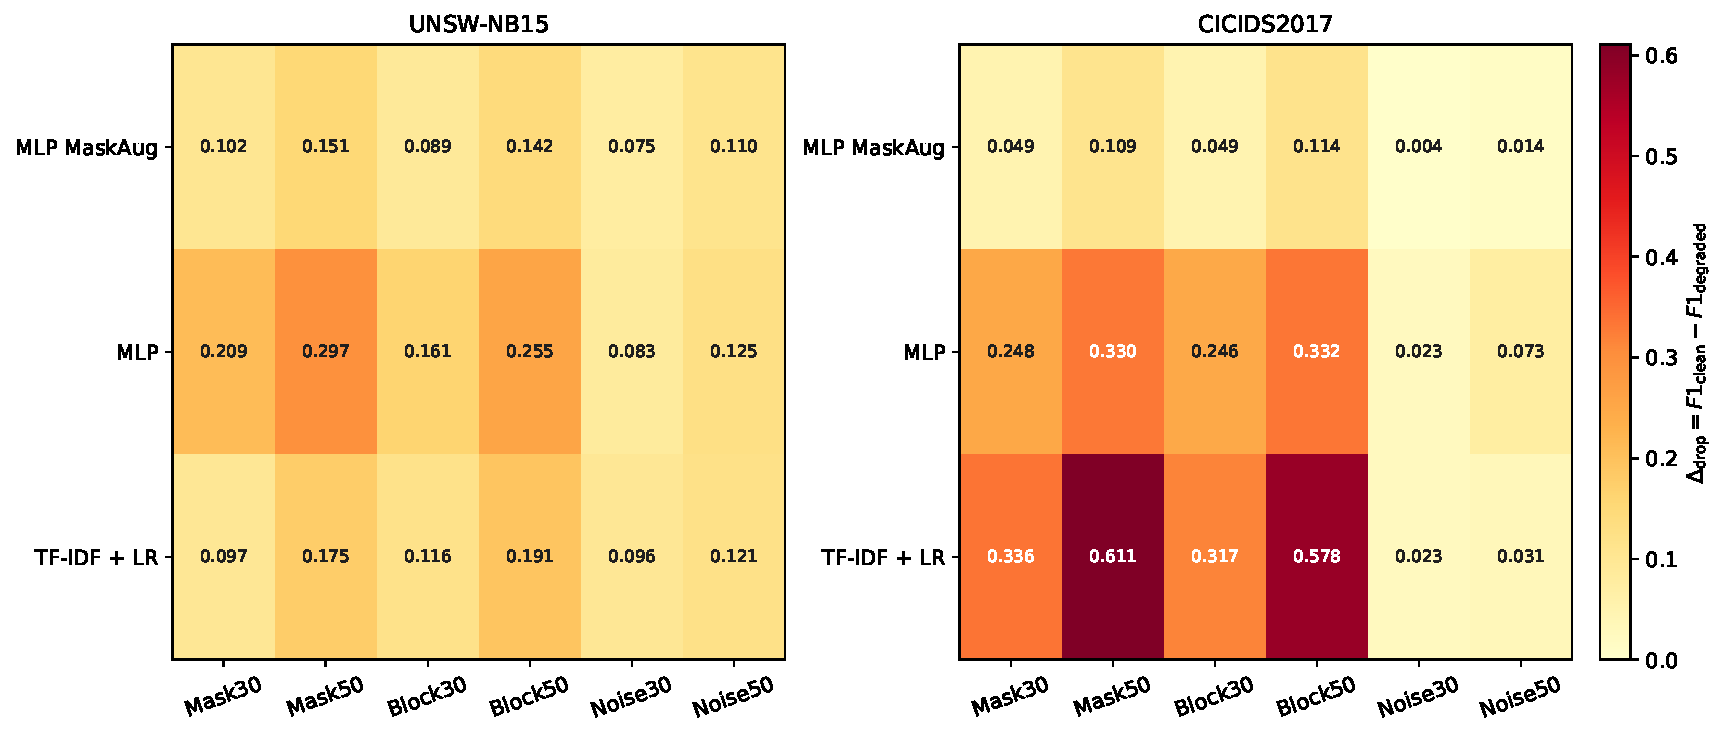
\includegraphics[width=\linewidth]{figures_appendix/relative_drop_from_clean.pdf}
    \caption{Heatmap view of performance drop from clean performance, defined as $\Delta_{\mathrm{drop}} = F1_{\mathrm{clean}} - F1_{\mathrm{degraded}}$. Smaller values indicate better robustness.}
    \label{fig:relative_drop}
\end{figure}

\begin{figure}[t]
    \centering
    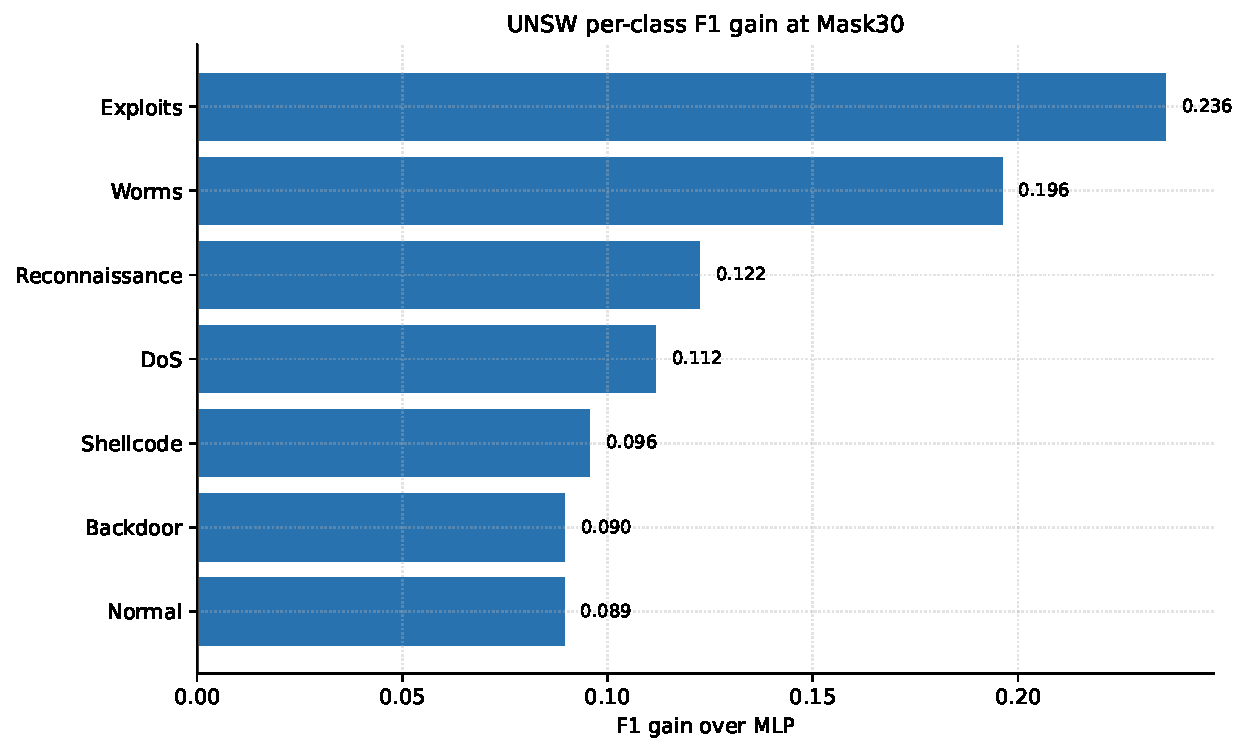
\includegraphics[width=\linewidth]{figures_appendix/per_class_f1_gain_mask30.pdf}
    \caption{Sorted per-class F1 gain of MLP MaskAug over the plain MLP at \texttt{Mask30} on UNSW-NB15, aggregated across model seeds.}
    \label{fig:per_class_f1_gain}
\end{figure}

\begin{figure}[t]
    \centering
    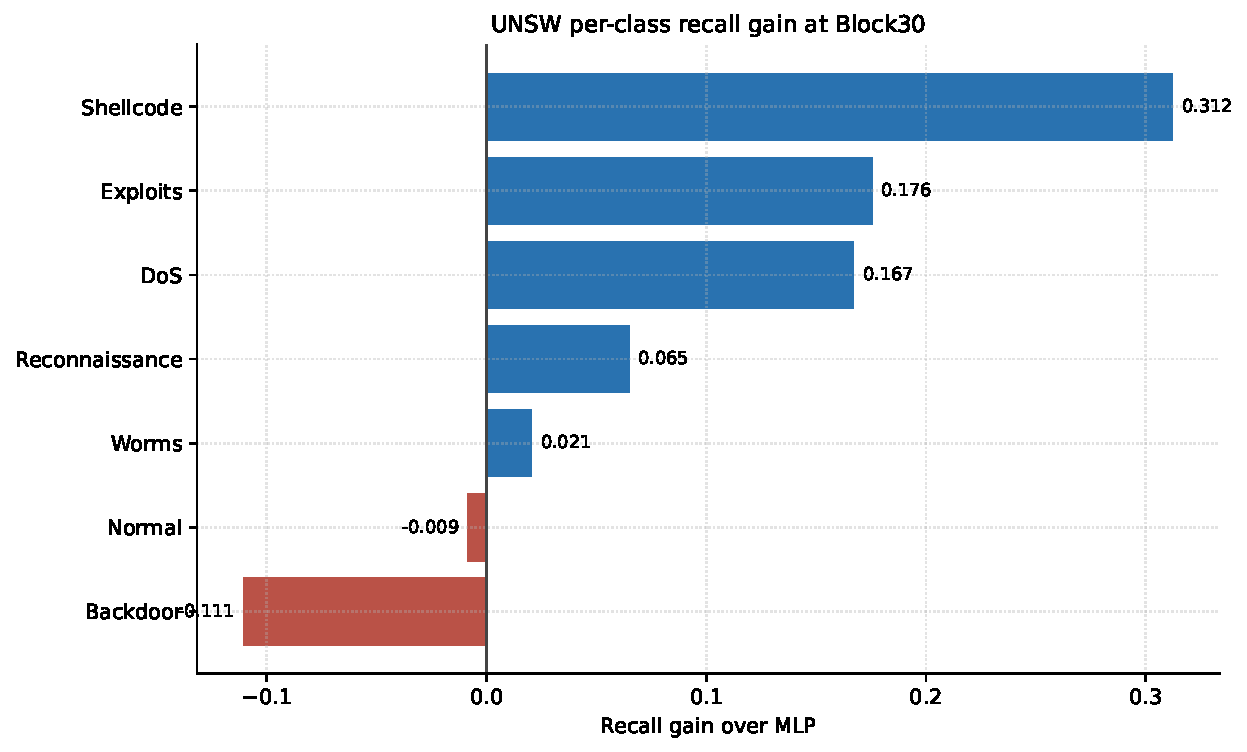
\includegraphics[width=\linewidth]{figures_appendix/per_class_recall_gain_block30.pdf}
    \caption{Sorted per-class recall gain of MLP MaskAug over the plain MLP at \texttt{Block30} on UNSW-NB15, aggregated across model seeds.}
    \label{fig:per_class_recall_gain}
\end{figure}

\begin{figure}[t]
    \centering
    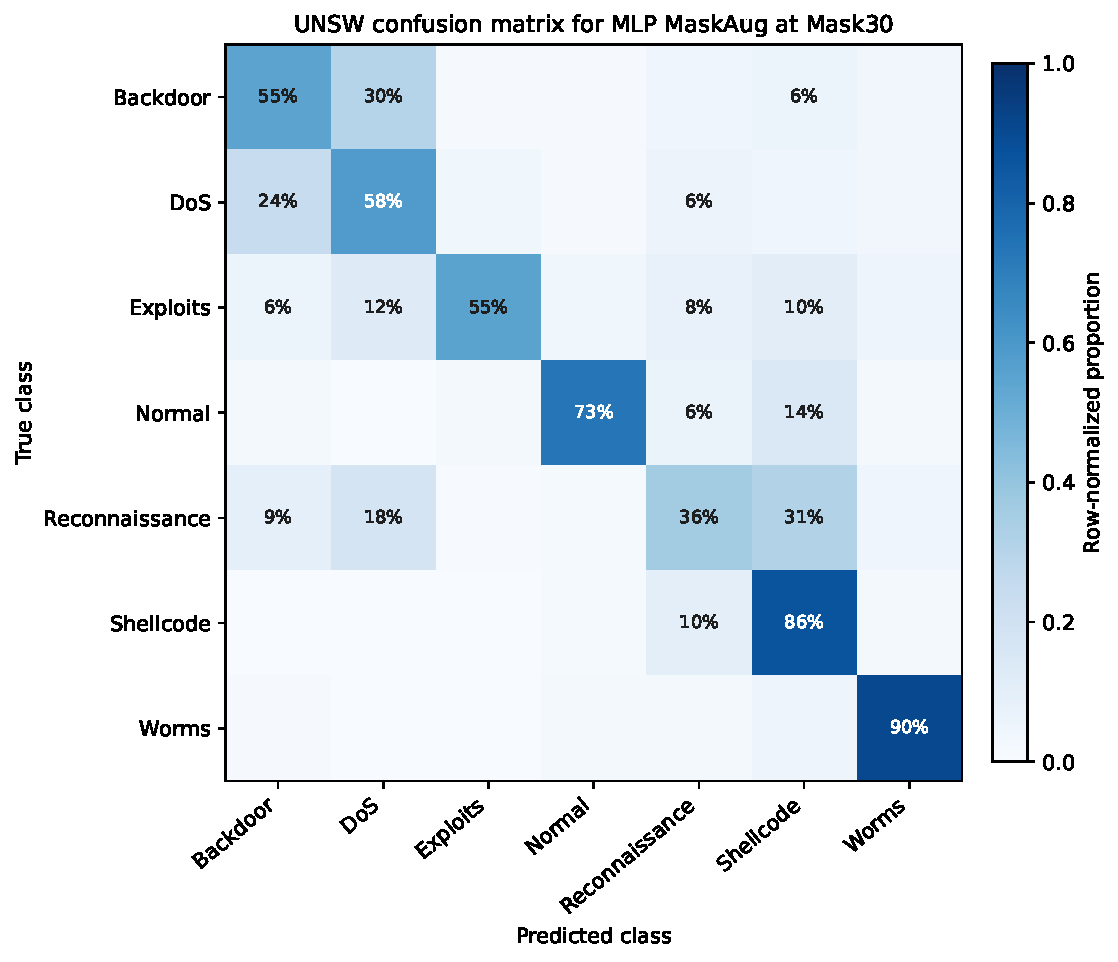
\includegraphics[width=0.82\linewidth]{figures_appendix/confusion_matrix_unsw_mask30.pdf}
    \caption{Row-normalized confusion matrix of MLP MaskAug at \texttt{Mask30} on UNSW-NB15, aggregated across model seeds.}
    \label{fig:cm_mask30}
\end{figure}

\section{Sensitivity Study}
Table~\ref{tab:sensitivity} reports the sensitivity sweep used to select the final augmentation policy. The final method is chosen by maximizing the four-condition mean among candidates that remain within 0.01 of the best clean score, which is why the Mask+Block+Noise configuration is retained as \texttt{MLP MaskAug} in the main text.

\begin{table}[t]
\centering
\caption{Sensitivity study for augmentation ratios on UNSW-NB15. The final method is selected by maximizing the four-condition mean among candidates within 0.01 of the best clean score.}
\label{tab:sensitivity}
\begin{tabular}{lccc}
\toprule
Candidate & Clean Macro-F1 & Mean\{Clean, Mask30, Block30, Noise30\} & Selected \\
\midrule
Mask+Block+Noise & 0.7017 & 0.6408 & Yes \\
Mask+Block & 0.7003 & 0.6364 & No \\
MaskOnly \{0.1,0.3\} & 0.6923 & 0.6345 & No \\
MaskOnly \{0.1,0.3,0.5\} & 0.6783 & 0.6280 & No \\
MaskOnly \{0.1\} & 0.6899 & 0.6207 & No \\
BlockOnly \{0.1\} & 0.6970 & 0.6111 & No \\
BlockOnly \{0.3\} & 0.6814 & 0.6015 & No \\
No augmentation & 0.6766 & 0.5634 & No \\
\bottomrule
\end{tabular}
\end{table}
